
\Literature: Sch{\"o}pfer \etal (2013) \cite{sccm13}.

A yield surface is a five-dimensional surface in the six-dimensional space of stresses. 
The state of stress of inside the yield surface is elastic. 
When the stress state lies on the surface the material is said to have reached its yield point 
and the material is said to have become plastic. Further deformation of the material causes 
the stress state to remain on the yield surface, even though the surface itself may change shape and 
size as the plastic deformation evolves, this is because stress states that lie outside the yield surface are non-permissible.

The yield surface is usually expressed in terms of (and visualized in) a three-dimensional principal 
stress space $(\sigma_1,\sigma_2,\sigma_3)$, a two- or three-dimensional space spanned by stress invariants 
or a version of the three-dimensional Haigh-Westergaard space\footnote{\url{https://en.wikipedia.org/wiki/Stress_space}}. 

\begin{center}
\includegraphics[width=14cm]{images/rheology/surfaces}\\
{\captionfont Yield surfaces in stress space \cite{zico74}. Note that 
the axes are $-\sigma_1$,$-\sigma_2$,$-\sigma_3$}
\end{center} 

Having obtained the equations for the yield functions in the previous sections, we can easily test
them as follows: in the ($\sigma_1$, $\sigma_2$, $\sigma_3$) space we can look for stress states 
that fulfil the yield equations. I set $c=20~\si{\mega\pascal}$ and $\phi=20$\degree and restrain 
the search to the space [-100~\si{\mega\pascal}:100~\si{\mega\pascal}]$^3$.
The python code and the gnuplot script used to generate the plots hereafter 
are in {\tt images/rheology/surfaces}. The implemented algorithm is somewhat  
naive and quite inefficient: discretise the space in $N^3$ points and for each point 
check whether any of the von Mises, Tresca, Mohr-Coulomb and (the three variants of) Drucker-Prager 
criteria is satisfied and when the point is in the space $\sigma_1+\sigma_2+\sigma_3=10$MPa 
(perpendicular to the $x=y=z$ line) write it to the corresponding file.

The recovered surfaces are similar to those of the figure above but their plot in a 3D space is difficult.
I have therefore isolated two sub-plots. 
The first one is for $\sigma_1=\sigma_2$:

\begin{center}
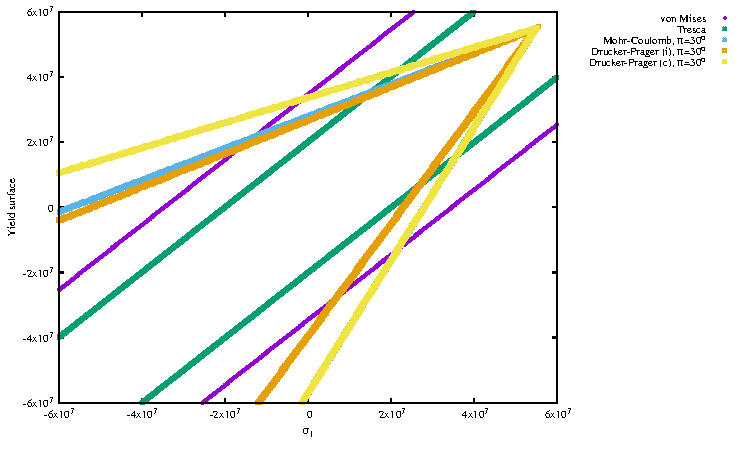
\includegraphics[width=12cm]{images/rheology/surfaces/res512/surfaces_xy.pdf}
\end{center}
We see that the von Mises and Tresca envelopes are parallel to the line $\sigma_1=\sigma_2=\sigma_3$ (which 
is expected since they do not depend on pressure).

The second plot is in the plane $\sigma_1+\sigma_2+\sigma_3=0$ which is perpendicular to the middle line 
$\sigma_1=\sigma_2=\sigma_3=0$. To facilitate plotting the envelopes are plotted as a function of $\sigma_1$ only (so that even though they are circles in the chosen plane they appear here as ellipses):

\begin{center}
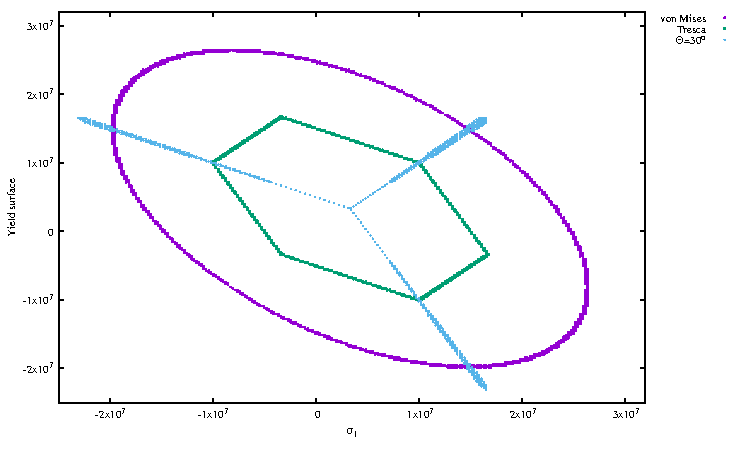
\includegraphics[width=14cm]{images/rheology/surfaces/res512/surfaces_plane2.pdf}\\
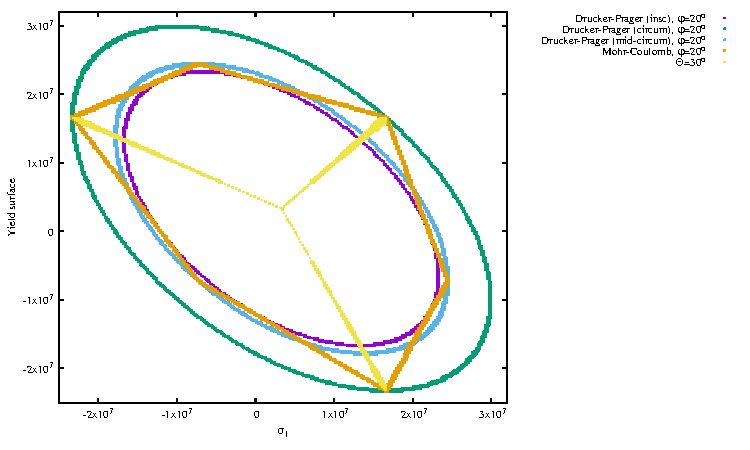
\includegraphics[width=14cm]{images/rheology/surfaces/res512/surfaces_plane.pdf}
\end{center}

We see that we indeed recover that the three Drucker-Prager formulations 
inscribe (purple), middle-circumscribe (blue) and circumscribe (green) the 
Mohr-Coulomb one. 

{\color{orange} the code for these plots has been moved to stone 159. Update necessary, etc ...}


